\documentclass{article}
\usepackage[utf8]{inputenc}
\usepackage[spanish]{babel}
\usepackage{listings}
\usepackage{graphicx}
\graphicspath{ {images/} }
\usepackage{cite}

\begin{document}

\begin{titlepage}
    \begin{center}
        \vspace*{1cm}
            
        \Huge
        \textbf{Parcial II 2021-1 Informática 2}
            
        \vspace{0.5cm}
        \LARGE
        Informe de Análisis y Diseño de la Solución del Desafío
            
        \vspace{1.5cm}
            
        \textbf{Juan Diego Cabrera Moncada}\\
            
        \vfill
            
        \vspace{0.8cm}
            
        \Large
        Despartamento de Ingeniería Electrónica y Telecomunicaciones\\
        Universidad de Antioquia\\
        Medellín\\
        Septiembre de 2021
            
    \end{center}
\end{titlepage}

\tableofcontents
\newpage
 \section{Análisis del problema y consideraciones para la alternativa de solución propuesta}
 En esta fase de análisis, al reconstruir el código que se había propuesto en clase, pude verificar que entendía en su totalidad el método de obtención de la información de cada pixel de una imagen en específico.
 \begin{figure}[h]
    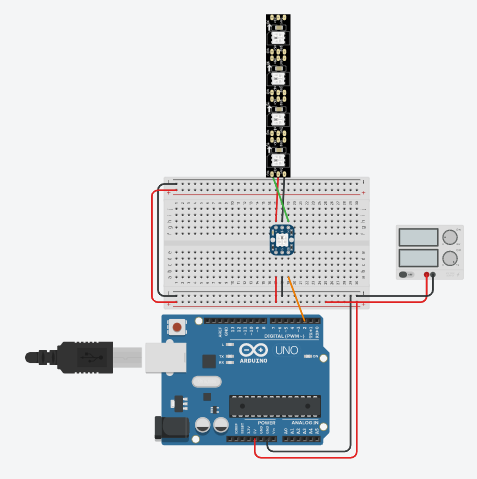
\includegraphics[width=10cm]{circ_pruebainicial.png}
    \centering
    \caption{Réplica del circuito propuesto en clase}
    \label{fig:replica_circInicial}
 \end{figure}
 Posterior a ello, asumí que el mayor problema en la programación sería hacer una función con la cual hiciese el proceso de submuestreo de una imagen, y otra similar, que hiciese el de sobremuestreo, en caso de que alguna de las dos sea necesaria. Para ello, en primer lugar, enfocándome en el submuestreo, pensé en que si obtenía el cociente de la división del ancho de la imagen entre el número de columnas de la matriz de Neopixeles o de LEDs, y de forma similar el alto entre el número de filas, para, posteriormente, usar dichos dos valores (Llamémoslos Cx y Cy), para hallar el promedio de un número Cx de valores (Teniendo en cuenta que pueden ser diferentes dependiendo de cúal de los 3 colores RGB esté analizando matricialmente) y así reducir ese número Cx a 1, y unir todas los valores resultantes hasta crear la versión submuestreada de la matriz. No obstante, al consultar opiniones al respecto en foros y otros sitios web, encontré que esto puede resultar inefectivo por cuestiones de que, hablando de un solo punto de la matriz, la distancia que habría entre los puntos de la matriz real que debe representar el punto de la matriz de submuestreo implica que unos puntos tengan más "peso" que otros al momento de hacer este proceso \cite{AplicarRemuestreo}. No obstante, uno de los comentarios \cite{Comm_ReduImg} proponía hacer el promedio de modo que se haga un submuestreo de reducir la matriz a la mitad en cada ejecución de la función, y, una vez se encuentre cerca de la matriz deseada, hacer la consideración de la influencia que tendría la distancia relativa entre un punto de la matriz real y el punto de la matriz de submuestreo que lo representa. Para garantizar una mejor resolución, he decidido optar por una matriz de 16 x 16 usando 16 tiras de 16 Neopixeles cada una. Por el momento, procedo a hacer una verificación de que el funcionamiento del código y el circuito está bien planteado para una matriz de Neopixeles de esta cantidad.
 \section{Esquema de tareas del desarrollo del algoritmo}
 En primer lugar, procedo a analizar la lista de tareas que se deben ejecutar para desarrollar el algoritmo de solución del desafío de manera efectiva. Analizando objetivos de forma secuencial, considero que, primero, es fundamental establecer el método de interacción con el usuario para solicitar la imagen a procesar, por lo cual, una parte de ello, consta de la creación del manual de uso del programa., que debe abordar a su vez, lo que debe hacer el usuario con el archivo de texto resultante del submuestreo o sobremuestreo de la imagen (En caso de que sea alguno de los 2 necesario), incluyendo cómo y dónde debe usarlo, pues dicho archivo contiene la información necesaria para que funcione correctamente la solución implementada en Tinkercad (Primera impresión de cómo debe conectarse Tinkercad y Qt). Una vez hechas las partes de interacción con el usuario, la siguiente tarea corresponde a crear un método de lectura de la información de la imagen y proveer una forma, mediante código, de guardar dicha información de modo que resulte cómoda de usar al procesarla para la cuestión de submuestreo o sobremuestreo de la imagen. Posterior a ello, debo definir métodos que me permitan manipular la información almacenada. Después, es necesario definir métodos, ciclos y ejecuciones necesarias para el caso en que se requiera realizar submuestreo de la imagen, en paralelo con aquellos necesarios para el caso de sobremuestreo de la imagen. Es necesario, después, garantizar métodos así para guardar la nueva información procesada de la imagen en conjunto con la manipulación del archivo de texto. Asimismo, otra tarea fundamental, la cual puede hacerse en paralelo con el proceso anteriormente descrito, radica en la construcción de la matriz de Neopixeles de modo que sea funcional, en primera instancia, y posterior a que ésto se garantice, priorizar la efectividad en la representación matricial de la información procesada de la imagen obtenida por vía del archivo de texto creado y modificado. Esta última tarea, se debe subdividir en la garantización de la representación matricial para cada uno de los colores RGB por separado como primer objetivo y, después, en conjunto.
 \section{Diseño del algoritmo}
 \section{Consideraciones a tener en cuenta en la implementación}
\bibliographystyle{IEEEtran}
\bibliography{references}

\end{document}